% ======================================================================
% fig_gain_headroom -- standalone build of a figure that main.tex also draws inline.
% ----------------------------------------------------------------------
% The tikzpicture below is copied VERBATIM from main.tex, so this file and
% the inline version render identically. Build with:
%     pdflatex fig_gain_headroom.tex
% The standalone class crops the PDF to the picture's bounding box, so no
% trim/clip is ever needed in the paper.
%
% Fonts: the picture inherits times/helvet, so every glyph is Type 1 and
% embedded by pdflatex. Nothing is rasterised, so DPI does not apply.
% ======================================================================
\documentclass[border=2pt]{standalone}

\usepackage{times}
\usepackage{helvet}
\usepackage{courier}
\usepackage{amsmath}
\usepackage{amssymb}
\usepackage{xcolor}
\usepackage{pifont}
\usepackage{tikz}
\usetikzlibrary{arrows.meta,positioning}

%% ======================================================================
%% preamble-figures.tex
%% ----------------------------------------------------------------------
%% Every definition the figures need, kept identical to main.tex's preamble.
%% Shared by the standalone builds in this folder; main.tex carries its own
%% copy so that the submitted source stays a single .tex file.
%% ======================================================================

\providecommand{\method}{\textsc{ESV}}

%% --- comparison-table glyphs (fig_trap uses \yes / \no) ---------------
\definecolor{okgreen}{RGB}{0,122,87}
\definecolor{okred}{RGB}{176,42,32}
\providecommand{\yes}{\textcolor{okgreen}{\ding{51}}}
\providecommand{\no}{\textcolor{okred}{\ding{55}}}
\providecommand{\na}{\textcolor{black!45}{--}}

%% --- figure fills, shaded by what each step costs ---------------------
\definecolor{cshared}{RGB}{226,226,226}
\definecolor{ccode}{RGB}{205,228,243}
\definecolor{ccall}{RGB}{252,230,192}
\definecolor{ccallb}{RGB}{191,118,0}
\definecolor{cout}{RGB}{206,238,227}
\definecolor{ctrap}{RGB}{250,222,218}

%% --- plot colours and markers -----------------------------------------
%% Marker shapes are core TikZ nodes, so every glyph is vector and uses the
%% document's Type 1 text fonts: no Type 3 subsets, no raster, nothing to crop.
\definecolor{pblue}{RGB}{31,97,160}
\definecolor{pgreen}{RGB}{0,122,87}
\definecolor{pgrey}{RGB}{95,95,95}
\providecommand{\mkopensq}[2]{\node[draw=#2,fill=white,line width=.6pt,rectangle,inner sep=1.5pt] at #1 {};}
\providecommand{\mkfillsq}[2]{\node[draw=#2,fill=#2,rectangle,inner sep=1.5pt] at #1 {};}
\providecommand{\mkopenci}[2]{\node[draw=#2,fill=white,line width=.6pt,circle,inner sep=1.5pt] at #1 {};}
\providecommand{\mkfillci}[2]{\node[draw=#2,fill=#2,circle,inner sep=1.5pt] at #1 {};}
%% #1 x, #2 centre, #3 half-width of the interval, #4 colour (needs x=1cm)
\providecommand{\ebar}[4]{%
  \draw[#4,line width=.5pt] (#1,{#2-#3}) -- (#1,{#2+#3});
  \draw[#4,line width=.5pt] ({#1-0.055},{#2-#3}) -- ({#1+0.055},{#2-#3});
  \draw[#4,line width=.5pt] ({#1-0.055},{#2+#3}) -- ({#1+0.055},{#2+#3});}

%% --- \cost is used inside the three schematic figures -----------------
\providecommand{\cost}{\scriptsize}


\begin{document}
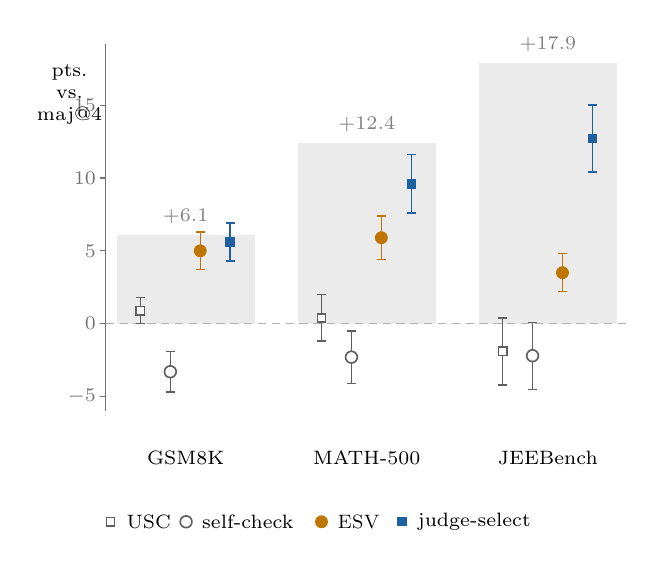
\begin{tikzpicture}[x=1cm, y=0.185cm, font=\footnotesize]
%% headroom: 0 up to the CoT pass@4 ceiling, the most any selector can gain
\fill[black!8] (0.70,0) rectangle (2.45,6.1);
\fill[black!8] (3.00,0) rectangle (4.75,12.4);
\fill[black!8] (5.30,0) rectangle (7.05,17.9);
\node[anchor=south, font=\scriptsize, black!50] at (1.575,6.2)  {$+6.1$};
\node[anchor=south, font=\scriptsize, black!50] at (3.875,12.5) {$+12.4$};
\node[anchor=south, font=\scriptsize, black!50] at (6.175,18.0) {$+17.9$};
%% axes
\draw[black!30, densely dashed] (0.56,0) -- (7.20,0);
\draw[black!55] (0.56,-6) -- (0.56,19.2);
\foreach \y in {-5,0,5,10,15}
  \draw[black!55] (0.49,\y) -- (0.56,\y) node[left=0pt, font=\scriptsize] {$\y$};
\node[anchor=south, font=\scriptsize, align=center] at (0.10,13.0) {pts.\\vs.\\maj@4};
%% benchmark labels
\node[font=\scriptsize] at (1.575,-9.2) {GSM8K};
\node[font=\scriptsize] at (3.875,-9.2) {MATH-500};
\node[font=\scriptsize] at (6.175,-9.2) {JEEBench};
%% ---- GSM8K
\ebar{1.00}{0.9}{0.9}{pgrey}   \mkopensq{(1.00,0.9)}{pgrey}
\ebar{1.38}{-3.3}{1.4}{pgrey}  \mkopenci{(1.38,-3.3)}{pgrey}
\ebar{1.76}{5.0}{1.3}{ccallb}  \mkfillci{(1.76,5.0)}{ccallb}
\ebar{2.14}{5.6}{1.3}{pblue}   \mkfillsq{(2.14,5.6)}{pblue}
%% ---- MATH-500
\ebar{3.30}{0.4}{1.6}{pgrey}   \mkopensq{(3.30,0.4)}{pgrey}
\ebar{3.68}{-2.3}{1.8}{pgrey}  \mkopenci{(3.68,-2.3)}{pgrey}
\ebar{4.06}{5.9}{1.5}{ccallb}  \mkfillci{(4.06,5.9)}{ccallb}
\ebar{4.44}{9.6}{2.0}{pblue}   \mkfillsq{(4.44,9.6)}{pblue}
%% ---- JEEBench
\ebar{5.60}{-1.9}{2.3}{pgrey}  \mkopensq{(5.60,-1.9)}{pgrey}
\ebar{5.98}{-2.2}{2.3}{pgrey}  \mkopenci{(5.98,-2.2)}{pgrey}
\ebar{6.36}{3.5}{1.3}{ccallb}  \mkfillci{(6.36,3.5)}{ccallb}
\ebar{6.74}{12.7}{2.3}{pblue}  \mkfillsq{(6.74,12.7)}{pblue}
%% legend
\mkopensq{(0.62,-13.6)}{pgrey} \node[anchor=west, font=\scriptsize] at (0.70,-13.6) {USC};
\mkopenci{(1.58,-13.6)}{pgrey} \node[anchor=west, font=\scriptsize] at (1.66,-13.6) {self-check};
\mkfillci{(3.30,-13.6)}{ccallb}\node[anchor=west, font=\scriptsize] at (3.38,-13.6) {\method{}};
\mkfillsq{(4.32,-13.6)}{pblue} \node[anchor=west, font=\scriptsize] at (4.40,-13.6) {judge-select};
\end{tikzpicture}
\end{document}
